\chapter{Önerme Mantığı}
\label{ch:propositional_logic}

Matematiksel önerme (proposition), doğru ya da yanlış olabilen bir ifadedir.
Bu bölüm \texttt{pytop.logic} modülünün sağladığı \texttt{Proposition},
bağlaçlar ve sonlu niceleyicileri tanıtır; ardından ayrılma aksiyomlarını
bu araçlarla nasıl ifade edebileceğimizi gösterir.

% -----------------------------------------------------------------------
\section{Önerme ve Doğruluk Değeri}
\label{sec:proposition}

\begin{definition}[Önerme]
Bir \textbf{önerme} (proposition), kesin bir doğruluk değerine sahip
(doğru veya yanlış) matematiksel bir ifadedir.
\end{definition}

\begin{lstlisting}[language=Python, caption={Temel önermeler}]
from pytop import (
    Proposition,
    negate, conjunction, disjunction, implies, iff,
    for_all, there_exists, unique_exists,
)

p = Proposition("p", True)
q = Proposition("q", False)

print(f"p : {p.truth_value}")
print(f"q : {q.truth_value}")
\end{lstlisting}

\begin{lstlisting}[style=output]
p : True
q : False
\end{lstlisting}

% -----------------------------------------------------------------------
\section{Mantıksal Bağlaçlar}
\label{sec:connectives}

\begin{table}[h]
\centering
\begin{tabular}{lll}
\toprule
\textbf{Fonksiyon} & \textbf{Sembol} & \textbf{Anlam} \\
\midrule
\texttt{negate(p)}        & $\neg p$       & p değil \\
\texttt{conjunction(p,q)} & $p \wedge q$   & p ve q \\
\texttt{disjunction(p,q)} & $p \vee q$     & p veya q \\
\texttt{implies(p,q)}     & $p \to q$      & p ise q \\
\texttt{iff(p,q)}         & $p \leftrightarrow q$ & p ancak ve ancak q \\
\bottomrule
\end{tabular}
\caption{pytop.logic bağlaç fonksiyonları}
\end{table}

\begin{lstlisting}[language=Python]
print("neg(p)  :", negate(p).truth_value)
print("p and q :", conjunction(p, q).truth_value)
print("p or q  :", disjunction(p, q).truth_value)
print("p -> q  :", implies(p, q).truth_value)
print("p <-> q :", iff(p, q).truth_value)
print("p <-> p :", iff(p, p).truth_value)
\end{lstlisting}

\begin{lstlisting}[style=output]
neg(p)  : False
p and q : False
p or q  : True
p -> q  : False
p <-> q : False
p <-> p : True
\end{lstlisting}

\texttt{implies(p, q)} yalnızca $p = \text{True},\ q = \text{False}$
durumunda yanlıştır; diğer üç kombinasyonda boş doğruluk (vacuous truth)
nedeniyle doğrudur.

Aşağıdaki görsel beş bağlacın dört satırlık doğruluk değerlerini bir arada
özetler: yeşil hücre \emph{doğru} (D), kırmızı hücre \emph{yanlış} (Y).

\begin{figure}[ht]
\centering
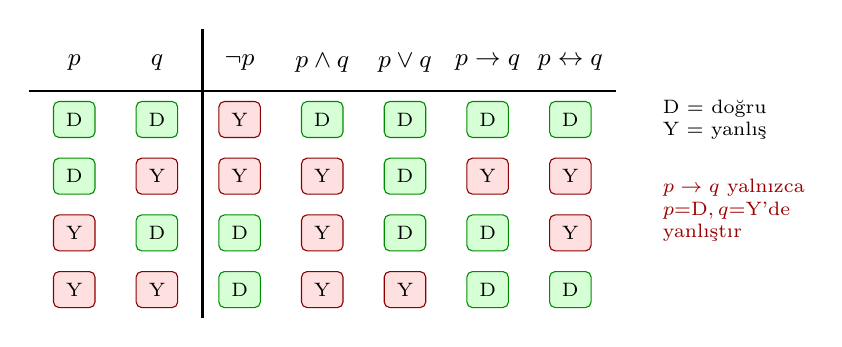
\begin{tikzpicture}[font=\small, x=1.05cm, y=0.72cm,
    D/.style={fill=green!16, draw=green!55!black, rounded corners=2pt,
              minimum width=15pt, minimum height=13pt},
    Y/.style={fill=red!12,  draw=red!55!black, rounded corners=2pt,
              minimum width=15pt, minimum height=13pt}]
  % --- Sutun basliklari ---
  \foreach \i/\lbl in {0/$p$, 1/$q$, 2/$\neg p$, 3/$p\wedge q$, 4/$p\vee q$, 5/$p\to q$, 6/$p\leftrightarrow q$} {
    \node[anchor=center] at (\i, 4) {\lbl};
  }
  % --- Baslik / sol blok ayrac cizgileri ---
  \draw[thick] (-0.55, 3.5) -- (6.55, 3.5);
  \draw[thick] (1.55, 4.6) -- (1.55, -0.5);

  % --- Satir 0: p=D q=D ---
  \node[D] at (0,3){\scriptsize D}; \node[D] at (1,3){\scriptsize D};
  \node[Y] at (2,3){\scriptsize Y}; \node[D] at (3,3){\scriptsize D};
  \node[D] at (4,3){\scriptsize D}; \node[D] at (5,3){\scriptsize D};
  \node[D] at (6,3){\scriptsize D};
  % --- Satir 1: p=D q=Y ---
  \node[D] at (0,2){\scriptsize D}; \node[Y] at (1,2){\scriptsize Y};
  \node[Y] at (2,2){\scriptsize Y}; \node[Y] at (3,2){\scriptsize Y};
  \node[D] at (4,2){\scriptsize D}; \node[Y] at (5,2){\scriptsize Y};
  \node[Y] at (6,2){\scriptsize Y};
  % --- Satir 2: p=Y q=D ---
  \node[Y] at (0,1){\scriptsize Y}; \node[D] at (1,1){\scriptsize D};
  \node[D] at (2,1){\scriptsize D}; \node[Y] at (3,1){\scriptsize Y};
  \node[D] at (4,1){\scriptsize D}; \node[D] at (5,1){\scriptsize D};
  \node[Y] at (6,1){\scriptsize Y};
  % --- Satir 3: p=Y q=Y ---
  \node[Y] at (0,0){\scriptsize Y}; \node[Y] at (1,0){\scriptsize Y};
  \node[D] at (2,0){\scriptsize D}; \node[Y] at (3,0){\scriptsize Y};
  \node[Y] at (4,0){\scriptsize Y}; \node[D] at (5,0){\scriptsize D};
  \node[D] at (6,0){\scriptsize D};

  \node[anchor=west, font=\scriptsize, align=left] at (7.0, 3.0)
    {D = doğru\\ Y = yanlış};
  \node[anchor=west, font=\scriptsize, align=left, red!60!black] at (7.0, 1.4)
    {$p\to q$ yalnızca\\ $p$=D,\,$q$=Y'de\\ yanlıştır};
\end{tikzpicture}

\caption{Beş temel bağlacın doğruluk tablosu: $\neg p$, $p\wedge q$,
$p\vee q$, $p\to q$, $p\leftrightarrow q$. $p\to q$ yalnızca tek satırda
($p$=D, $q$=Y) yanlıştır.}
\label{fig:ch02_baglac_dogruluk}
\end{figure}

\begin{sezgi}
Bağlaçları ``kapı'' olarak düşünün. $\wedge$ (ve) her iki girdi de doğruyken
akım geçirir; $\vee$ (veya) en az biri doğru olunca geçirir; $\to$ (ise)
yalnızca ``doğru bir öncülden yanlış bir sonuç'' çıkarılırsa kapanır. İşte bu
yüzden $p\to q$ sütununda yalnızca tek bir satır ($p$=D, $q$=Y) yanlıştır —
diğer her şey, mantığın ``verdiğin sözü bozmadın'' kuralıdır.
\end{sezgi}

\begin{karsiornek}
$p\to q$ ile $p\leftrightarrow q$ aynı şey değildir. $p$=Y, $q$=D alındığında
$p\to q$ \textbf{doğru} (D), ama $p\leftrightarrow q$ \textbf{yanlış} (Y)
döner: içerme tek yönlüdür, çift-koşul iki yönü birden ister.
\end{karsiornek}

% -----------------------------------------------------------------------
\section{Algoritmalar}
\label{sec:logic_algorithms}

\subsection{Doğruluk Tablosu Üretimi}

\begin{algorithm}
\caption{Doğruluk Tablosu (İki Değişkenli)}
\label{alg:truth_table}
\begin{algorithmic}[1]
\Require Bağlaç fonksiyonu $f$
\Ensure Dört satırlı doğruluk tablosu
\For{$(t_p, t_q) \in \{(T,T),(T,F),(F,T),(F,F)\}$}
  \State $p \leftarrow \text{Proposition}("p", t_p)$
  \State $q \leftarrow \text{Proposition}("q", t_q)$
  \State Yazdır $(t_p, t_q, f(p, q).\text{truth\_value})$
\EndFor
\end{algorithmic}
\end{algorithm}

\subsection{Tautoloji Denetimi}

Bir $\phi(p_1,\ldots,p_n)$ formülü tautoloji iff tüm $2^n$ atama için
doğrudur — $O(2^n \cdot |\phi|)$.

% -----------------------------------------------------------------------
\section{pytop API}
\label{sec:logic_api}

\begin{lstlisting}[language=Python, caption={logic modülü importu}]
from pytop import (
    Proposition,
    negate, conjunction, disjunction, implies, iff,
    for_all, there_exists, unique_exists,
)
\end{lstlisting}

Niceleyiciler:
\begin{lstlisting}[language=Python]
for_all(carrier, predicate)       # tum x: P(x)
there_exists(carrier, predicate)  # bazi x: P(x)
unique_exists(carrier, predicate) # tam bir x: P(x)
\end{lstlisting}

% -----------------------------------------------------------------------
\section{Örnekler}
\label{sec:logic_examples}

\subsection{Doğruluk Tablosu}

\begin{lstlisting}[language=Python]
pairs = [(True, True), (True, False), (False, True), (False, False)]
print(f"{'p':>5}  {'q':>5}  {'neg_p':>5}  {'p&q':>5}  {'p|q':>5}  {'p->q':>6}  {'p<->q':>6}")
for tv_p, tv_q in pairs:
    pp = Proposition("p", tv_p)
    qq = Proposition("q", tv_q)
    row = (pp.truth_value, qq.truth_value,
           negate(pp).truth_value, conjunction(pp, qq).truth_value,
           disjunction(pp, qq).truth_value,
           implies(pp, qq).truth_value, iff(pp, qq).truth_value)
    print("  ".join(f"{str(v):>5}" for v in row))
\end{lstlisting}

\begin{lstlisting}[style=output]
    p      q  neg_p    p&q    p|q   p->q  p<->q
----------------------------------------------------
 True   True  False   True   True   True   True
 True  False  False  False   True  False  False
False   True   True  False   True   True  False
False  False   True  False  False   True   True
\end{lstlisting}

\subsection{Tautolojiler — De Morgan ve Karşıt}

\begin{theorem}[De Morgan Yasaları]
\label{thm:de_morgan}
\begin{align*}
\neg(p \wedge q) &\leftrightarrow \neg p \vee \neg q \\
\neg(p \vee q) &\leftrightarrow \neg p \wedge \neg q
\end{align*}
\end{theorem}

\begin{theorem}[Karşıt (Contrapositive)]
\label{thm:contrapositive}
$(p \to q) \leftrightarrow (\neg q \to \neg p)$
\end{theorem}

En sık yapılan mantık hatası, bir içermeyi \textbf{tersiyle (converse)}
karıştırmaktır. $p\to q$'nin doğru biçimde denk olduğu ifade
\emph{kontrapozitiftir}: $\neg q\to\neg p$. Buna karşılık $q\to p$ (tersi)
genellikle denk \emph{değildir}.

\begin{figure}[ht]
\centering
\begin{tikzpicture}[font=\small, node distance=11mm,
    box/.style={draw, rounded corners, fill=blue!7, inner sep=6pt, minimum width=20mm},
    denk/.style={draw=green!55!black, rounded corners, fill=green!8, inner sep=6pt, minimum width=20mm}]

  % --- Ust satir: dogru denklik p->q  <=>  ¬q->¬p ---
  \node[box]  (pq)  {$p \to q$};
  \node[denk, right=28mm of pq] (cp) {$\neg q \to \neg p$};
  \draw[{Stealth[length=2.6mm]}-{Stealth[length=2.6mm]}, thick, green!45!black]
    (pq) -- node[above=1pt, font=\scriptsize, green!45!black] {denk} (cp);
  \node[font=\scriptsize, green!45!black, above=9mm] at ($(pq)!0.5!(cp)$) {kontrapozitif};

  % --- Alt satir: yanlis denklik p->q  ⇏  q->p ---
  \node[box, below=20mm of pq]  (pq2)  {$p \to q$};
  \node[box, right=28mm of pq2] (qp)   {$q \to p$};
  \draw[{Stealth[length=2.6mm]}-{Stealth[length=2.6mm]}, thick, red!65!black, dashed]
    (pq2) -- node[below=1pt, font=\scriptsize, red!65!black] {denk \emph{değil}} (qp);
  \node[font=\scriptsize, red!65!black, below=9mm] at ($(pq2)!0.5!(qp)$)
    {tersi (converse) — yaygın hata};

  % --- Karsi-ornek aciklamasi ---
  \node[anchor=west, font=\scriptsize, align=left, draw=red!40, fill=red!4,
        rounded corners, inner sep=5pt] at (6.7, -1.45)
    {Karşı-örnek: $p$=``kare'', $q$=``dikdörtgen''.\\
     $p\to q$ doğru, ama $q\to p$ yanlış\\
     (her dikdörtgen kare değildir).};
\end{tikzpicture}

\caption{Kontrapozitif denkliği $p\to q \Leftrightarrow \neg q\to\neg p$
(yeşil) ile denk \emph{olmayan} tersi $q\to p$ (kırmızı kesikli).}
\label{fig:ch02_kontrapozitif}
\end{figure}

\begin{karsiornek}
$p$ = ``$x$ bir karedir'', $q$ = ``$x$ bir dikdörtgendir'' olsun. $p\to q$
doğrudur (her kare dikdörtgendir), ama tersi $q\to p$ yanlıştır (her dikdörtgen
kare değildir). Kontrapozitif $\neg q\to\neg p$ = ``dikdörtgen değilse kare de
değildir'' ise yine doğrudur — çünkü o $p\to q$ ile denktir.
\end{karsiornek}

\paragraph{İspat eskizi (kontrapozitif).}
$p\to q$ ile $\neg q\to\neg p$ aynı doğruluk sütununu üretir; dört satırda da
çakışırlar, dolayısıyla $(p\to q)\leftrightarrow(\neg q\to\neg p)$ tautolojidir.
\[
\begin{array}{cc|cc}
p & q & p\to q & \neg q\to\neg p \\ \hline
\text{D} & \text{D} & \text{D} & \text{D} \\
\text{D} & \text{Y} & \text{Y} & \text{Y} \\
\text{Y} & \text{D} & \text{D} & \text{D} \\
\text{Y} & \text{Y} & \text{D} & \text{D}
\end{array}
\]

\paragraph{İspat eskizi (De Morgan).}
$p\wedge q$ yalnızca her ikisi doğruyken doğrudur; öyleyse $\neg(p\wedge q)$
``en az biri yanlış'' demektir. $\neg p\vee\neg q$ de tam olarak bunu söyler.
İki sütun her atamada çakıştığından $\neg(p\wedge q)\leftrightarrow\neg p\vee\neg q$
tautolojidir; ikincil yasa $\neg(p\vee q)\leftrightarrow\neg p\wedge\neg q$
$\wedge$ ile $\vee$ rolleri değiştirilerek aynı şekilde gösterilir.
\[
\begin{array}{cc|ccc}
p & q & p\wedge q & \neg(p\wedge q) & \neg p\vee\neg q \\ \hline
\text{D} & \text{D} & \text{D} & \text{Y} & \text{Y} \\
\text{D} & \text{Y} & \text{Y} & \text{D} & \text{D} \\
\text{Y} & \text{D} & \text{Y} & \text{D} & \text{D} \\
\text{Y} & \text{Y} & \text{Y} & \text{D} & \text{D}
\end{array}
\]

\begin{lstlisting}[language=Python]
def check_tautology(name, func):
    ok = all(func(Proposition("p", tp), Proposition("q", tq)).truth_value
             for tp, tq in [(True,True),(True,False),(False,True),(False,False)])
    print(f"{name}: {'tautoloji' if ok else 'DEGIL'}")

check_tautology("neg(p&q) <-> neg_p|neg_q",
    lambda p, q: iff(negate(conjunction(p, q)), disjunction(negate(p), negate(q))))
check_tautology("(p->q) <-> (neg_q->neg_p)",
    lambda p, q: iff(implies(p, q), implies(negate(q), negate(p))))
\end{lstlisting}

\begin{lstlisting}[style=output]
neg(p&q) <-> neg_p|neg_q: tautoloji
(p->q) <-> (neg_q->neg_p): tautoloji
\end{lstlisting}

\subsection{Niceleyiciler}

\begin{lstlisting}[language=Python]
X = [1, 2, 3, 4, 5]
print("for_all(X, x>0)       :", for_all(X, lambda x: x > 0))
print("for_all(X, x>2)       :", for_all(X, lambda x: x > 2))
print("there_exists(X, x>4)  :", there_exists(X, lambda x: x > 4))
print("unique_exists(X, x==3):", unique_exists(X, lambda x: x == 3))
\end{lstlisting}

\begin{lstlisting}[style=output]
for_all(X, x>0)       : True
for_all(X, x>2)       : False
there_exists(X, x>4)  : True
unique_exists(X, x==3): True
\end{lstlisting}

\subsection{Topoloji Uygulaması — T0 ve T1}

\begin{definition}[T0 — Kolmogorov]
$\forall x \neq y \in X,\ \exists$ açık $U : (x \in U,\ y \notin U)$ veya
$(y \in U,\ x \notin U)$.
\end{definition}

\begin{definition}[T1 — Fréchet]
$\forall x \neq y \in X,\ \exists$ açık $U : x \in U,\ y \notin U$.
\end{definition}

\begin{lstlisting}[language=Python]
from pytop import sierpinski_space, discrete_topology, indiscrete_topology

def is_t0_logic(space):
    pts   = list(space.carrier)
    opens = list(space.topology)
    return for_all(
        [(x, y) for x in pts for y in pts if x != y],
        lambda pair: there_exists(
            opens, lambda U: (pair[0] in U) != (pair[1] in U)
        )
    )

def is_t1_logic(space):
    pts   = list(space.carrier)
    opens = list(space.topology)
    return for_all(
        [(x, y) for x in pts for y in pts if x != y],
        lambda pair: there_exists(
            opens, lambda U: pair[0] in U and pair[1] not in U
        )
    )

for name, sp in [("Sierpinski", sierpinski_space()),
                 ("Discrete  ", discrete_topology(0, 1)),
                 ("Indiscrete", indiscrete_topology(0, 1))]:
    print(f"{name}  T0={is_t0_logic(sp)}  T1={is_t1_logic(sp)}")
\end{lstlisting}

\begin{lstlisting}[style=output]
Sierpinski  T0=True   T1=False
Discrete    T0=True   T1=True
Indiscrete  T0=False  T1=False
\end{lstlisting}

% -----------------------------------------------------------------------
\section{Alıştırmalar}
\label{sec:logic_exercises}

\begin{enumerate}
  \item Beş önerme değeriyle tam bir doğruluk tablosu oluşturun; \texttt{implies}
        kaç \texttt{(p, q)} çiftinde \texttt{False} döner?

  \item \texttt{unique\_exists([0,1,2,3,4], predicate)} değerini \texttt{True}
        yapan üç farklı koşul yazın.

  \item T2 (Hausdorff) aksiyomunu \texttt{for\_all} ve \texttt{there\_exists}
        kullanarak kodlayın:
        $\forall x \neq y,\ \exists$ açık $U,V : x \in U,\ y \in V,\ U \cap V = \emptyset$.
        Sierpiński, discrete ve indiscrete için test edin.

  \item \textit{(Teori)} \texttt{implies(p, q)} neden yalnızca $p = T, q = F$
        durumunda yanlıştır? Boş doğruluk (vacuous truth) kavramını açıklayın.

  \item \textit{(Teori)} De Morgan yasalarını önerme mantığı için ispatlayın:
        $\neg(p \wedge q) \leftrightarrow \neg p \vee \neg q$.

  \item \texttt{check\_tautology} yardımcı fonksiyonunu kullanarak
        \textbf{dağılma yasasını} doğrulayın:
        $p \wedge (q \vee r) \leftrightarrow (p \wedge q) \vee (p \wedge r)$.
        Üç değişken olduğundan sekiz $(p, q, r)$ atamasının tümünü gezmeniz
        gerekir; \texttt{iff}'in her atamada \texttt{True} döndüğünü gösterin.

  \item \textit{(Teori)} Bir öğrenci ``$p \to q$ doğruysa $q \to p$ de
        doğrudur'' diyor. Bu iddianın neden yanlış olduğunu, kontrapozitif
        $\neg q \to \neg p$ ile tersi $q \to p$ arasındaki farkı vurgulayan
        somut bir karşı-örnekle açıklayın. \ipucu{$p$ = ``tam sayı 4'e bölünür'',
        $q$ = ``tam sayı çifttir''.}
\end{enumerate}
